\begin{subfigure}[b]{0.475\textwidth}
        \centering
        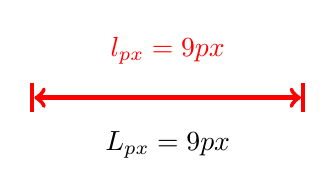
\begin{tikzpicture}
	    \foreach \line [count=\y] in \pixelsHorizontal {
    			\foreach \pix [count=\x] in \line {
      			\draw[fill=pixel \pix] (\x/\scaleSmall,-\y/\scaleSmall) rectangle +(1/								\scaleSmall,1/\scaleSmall);
    			}
  		}
  		\draw[ultra thick,|<->|,red] (0.85,-1.4) -- (4.35,-1.4);
  		\draw (2.6,-.8) node[red,ultra thick,fill=white] {$l_{\text{px}}=\SI{9}{px}$};
  		\draw (2.6,-2) node[black,ultra thick,fill=white] {$L_{\text{px}}=\SI{9}{px}$};
        \end{tikzpicture}
        \caption{Hier entspricht die Länge der Pixel genau der zugrundeliegenden Linie ($\SI{1}{Pixel} \equiv \SI{1}{px}$)}
        \label{fig:pixelHorizontal}
    \end{subfigure}
    \hfill
    \begin{subfigure}[b]{0.475\textwidth}
        \centering
        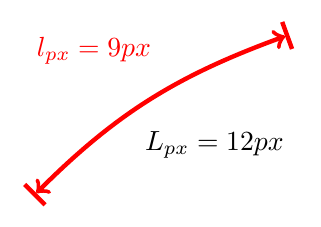
\begin{tikzpicture}[label distance=10mm]
        \foreach \line [count=\y] in \pixelsDiagonal {
    			\foreach \pix [count=\x] in \line {
      			\draw[fill=pixel \pix] (\x/\scaleSmall,-\y/\scaleSmall) rectangle +(1/								\scaleSmall,1/\scaleSmall);
    			}
  		}
  		\coordinate (A) at (0.6,-2.65);
  		\coordinate (B) at (3.85,-.6);
  		\draw [red,ultra thick,|<->|]   (A) to[out=45,in=200] (B);
  		\draw (1.37,-.8) node[red,ultra thick,fill=white] {$l_{\text{px}}=\SI{9}{px}$};
  		\draw (2.9,-2.0) node[black,ultra thick,fill=white] {$L_{\text{px}}=\SI{12}{px}$};
        \end{tikzpicture}
        \caption{Dieses kurvige Bogenstück ist ein Ausschnitt der Kontur aus Abb. \ref{fig:kante} ($\SI{1}{Pixel} \equiv \SI{0.7}{px}$) }
        \label{fig:pixelDiagonal}
    \end{subfigure}